\section{Design} \label{sec:design}

This section describes the requirements of the database, and how the Entity 
Relation diagram was designed to facilitate those requirements. 

\subsection{Requirements}

We want our database to be compatible for storing train systems and planning 
routes. Therefore we want parts of our database relations to easily resemble 
graph structures. These ``graph'' relations are specifically \emph{Station}, 
\emph{Route}, \emph{Track}, and \emph{RouteTracks}.

That is, \emph{Station} can be seen as the relation containing vertices, and 
\emph{Track} containing the edges between vertices. \emph{RouteTracks} then 
contains a composition of tracks/edges to resemble a route that connects 
through different stations/vertices.

The other relations like \emph{Train}, \emph{Employees} and \emph{Shift} are 
not really key parts of our database functionality, but are relations that 
should be included none the less.

As general description of our desired database is as follows:
The train management system i organized into stations. Stations have a number 
of lanes, and are located in cities. Stations are connected to each other with 
tracks. A track therefore always have a station in each of its endpoints and 
has a given length. Routes have a start and stop station. A route is composed 
of multiple tracks, and spans over several stations. The length of a route 
should be possible to calculate from its tracks contained.

A train can ride on an existing route. There is no limit for the amount of trains driving at the same time. A train has a model, production year and an age. An employee can have a work shift on a train, and the shift has a start time and end time. An employee has unique initials, a name, and an address.

\subsection{Functionality}
% Functional requirements:
% Views:
%  * Length of a route
%  * View stations on a route
% Functions / Triggers / ... Mention functionality of those (NOT how they were 
% implemented)
There are certain functionalities that we want our \emph{Train Management} 
schema to have, and these functionalities are what should define our schema as 
being a database for managing train systems and planning routes.

These functionalities are accomplished with the use of views, functions, 
triggers, procedures, etc.

Some of the most essential functionalities we want our database to have is
\begin{itemize}
\item Be able to find the length of a route.
\item Be able to find the stations on a route.
\item Data integrity
\item Compatibility for depth search algorithms and shortest routes algorithms.
\end{itemize}

Fortunately, simple views can be used to easily find the length of a route and its stations. These views are describes in the implementation section. So is a trigger that helps with data integrity of station lanes, by preventing illegal inserts. The compatibility for applying graph algorithms is achieved with the design of our relations, shown on the ER diagram Figure~\ref{fig:ER}.

\subsection{ER diagram}
Figure~\ref{fig:ER} shows our ER diagram, which illustrates the design of our 
\emph{Train Management} schema. It shows that some entities have total 
participation in some of the relations, as for instance you can not have tracks 
without stations or cities, neither can you have routes without tracks.

\begin{figure}[ht!]
    \centering
    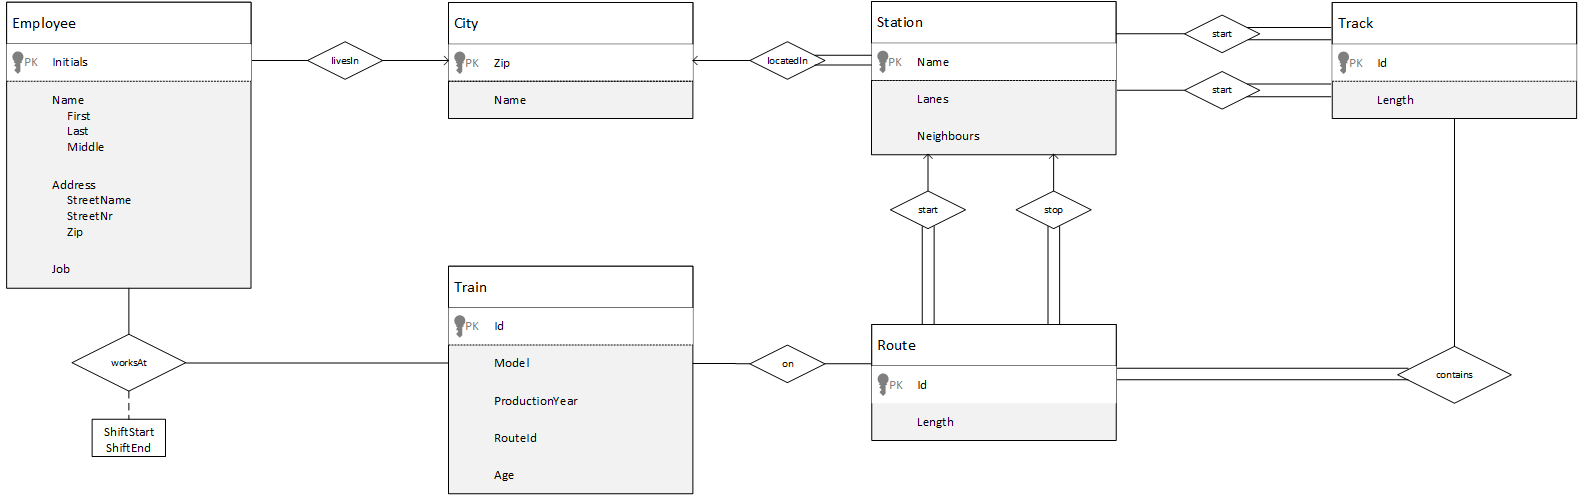
\includegraphics[angle=90,origin=c,width=.45\textwidth]{img/Handwritten_ER}
    \caption{An ER diagram depiction the design of the database}
    \label{fig:ER}
\end{figure}

% Design coices 
% See notes on hand drawn ER diagram (marked by *) None of those 3 examples 
% have been mentioned

% Comments on ER diagram supporting the requirements
The relations \emph{Station} and \emph{Track} are purposely designed to resemble "graph" relations as described in the requirements. This enables the possible implementation of graph-algorithms, with \emph{Stations} being nodes/vertices and \emph{Track} as edges.

Further functionalities and advancements could have been done in the form of including timestamps and time as a general factor for route-planning etc. Due to the scale of the project and keeping it realistically achievable at the same time, it has been decided to not include time in any form, other than the workshift start and end times. We considered letting the \emph{RouteTracks} relation have its own attribute called StopAt, which would specify which stations a route would stop at and when. However, for simplicity we decided to just have a route stop at every station on its path instead.\\
The ER diagram shows total participation between \emph{Route} and 
\emph{RouteTracks}. This however is really tricky to have implemented in the 
SQL Schema. In fact it is not implemented in the current schema. This is discussed in the implementation section.
